%!TEX root = ../thesis.tex
%*******************************************************************************
%****************************** Sixth Chapter **********************************
%*******************************************************************************
\chapter{Implementation}

\graphicspath{{Chapter6/Figs/Raster/}{Chapter6/Figs/PDF/}{Chapter6/Figs/}}

\begin{figure}[!ht] 
    \centering    
    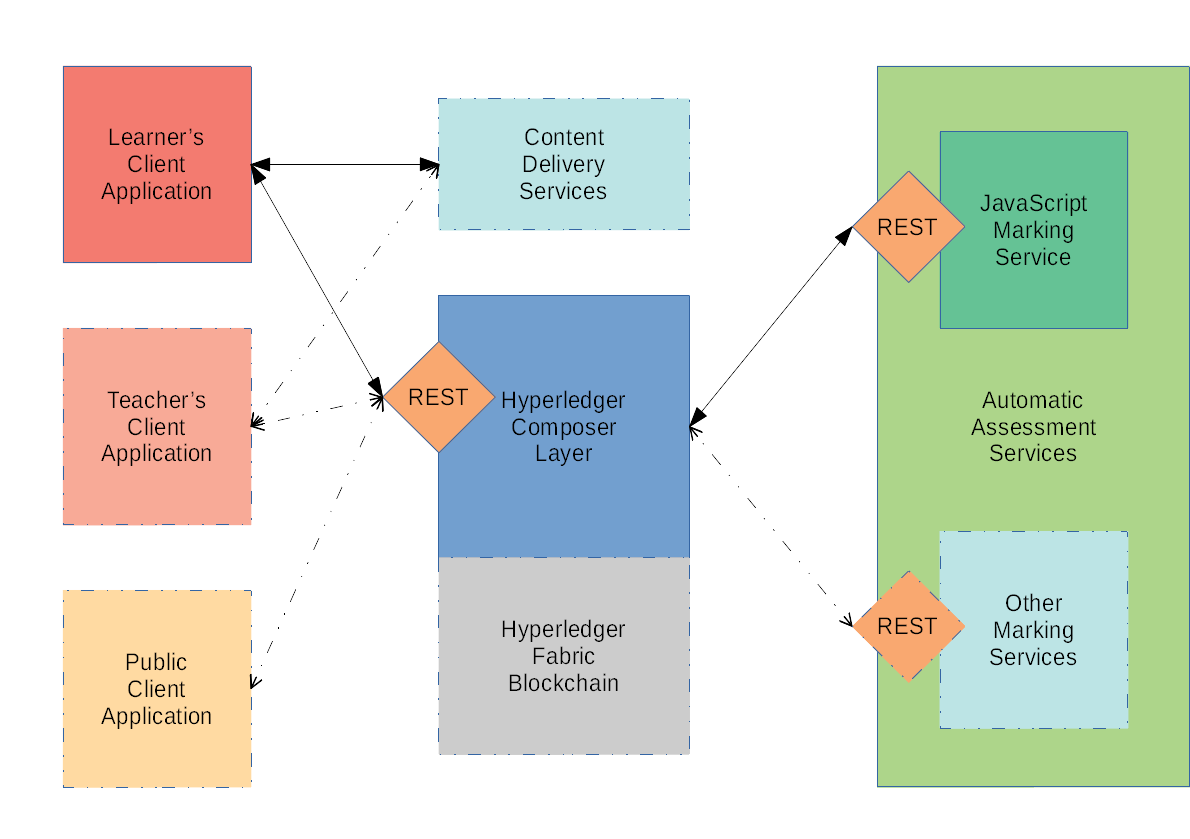
\includegraphics[width=1.0\textwidth]{architecture}
    \caption[Technical architecture overview for the demonstrator system built]
        {Technical architecture overview for the demonstrator system built}
    \label{fig:architecture}
\end{figure} 

\section{Tech Stack and Development Tools}

To prevent blah, version control was applied to 
GitHub is a git-based version control, code hosting and project management service that offers free 
private repositories to verified students \citep{github2018education}.

\begin{figure}[!hb] 
    \centering    
    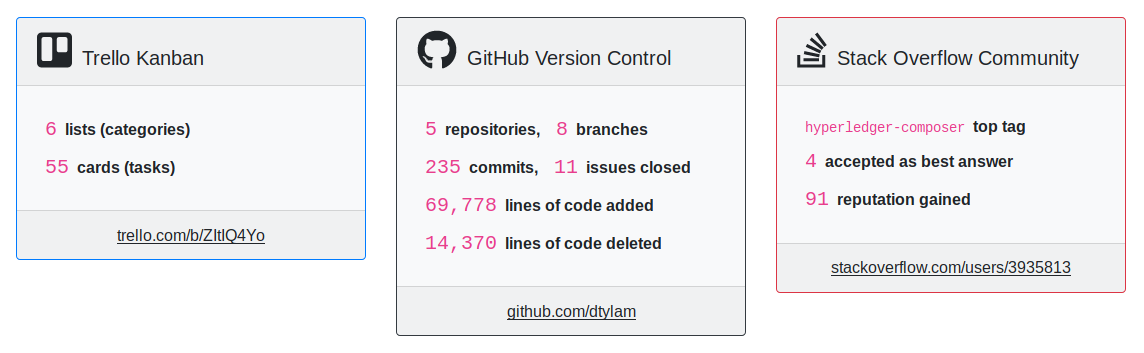
\includegraphics[width=1.0\textwidth]{platforms_stats}
    \caption[Project Management Statistics]
        {Statistics from Trello, GitHub and Stack Overflow collected over the duration of this project} 
    \label{fig:platforms_stats}
\end{figure}

\section{CLI and API}

\section{Learner Client Application}

\section{Teacher Client Application}

\section{Testing}